\documentclass[12pt]{article}
\usepackage[utf8]{inputenc}
\usepackage[T1]{fontenc}
\usepackage{lmodern}
\usepackage{geometry}
\usepackage{graphicx}
\usepackage{amsmath, amssymb}
\usepackage{booktabs}
\usepackage{hyperref}
\usepackage{tikz}
\usepackage{xcolor}
\usepackage{array}
\usepackage{enumitem}
\usepackage{fancyhdr}
\usepackage{setspace}

\geometry{margin=1in}
\setstretch{1.15}
\setlist[itemize]{leftmargin=1.5em}
\setlist[enumerate]{leftmargin=1.5em}

\pagestyle{fancy}
\fancyhf{}
\lhead{PDF OCR Stress Test}
\rhead{\thepage}

\title{\textbf{OCR Stress Test Document}\\\large Mixed content for PDF~$\rightarrow$~Image~$\rightarrow$~Text validation}
\author{pdfocr Project}
\date{\today}

\begin{document}
\maketitle

\begin{abstract}
This document intentionally mixes plain text, mathematical notation, tables, lists, vector drawings, and hyperlinks. It is meant to probe how well the OCR pipeline handles varied layouts, line breaks, and semantic structure.
\end{abstract}

\section{Overview}
The following sections combine narrative text with display math and inline symbols such as $E = mc^2$, $\nabla \cdot \vec{E} = \rho / \varepsilon_0$, and probability notation $\mathbb{P}(X \leq x)$. Paragraphs use hyphenation and line wraps to stress layout-aware OCR. Repeated words with subtle differences (e.g., \emph{kernel} vs. \emph{kernels}) are present to spot hallucinations.

\section{Display Mathematics}
We include a few multi-line expressions to check alignment:
\begin{align}
f(x) &= \int_{-\infty}^{\infty} e^{-t^2} \, dt = \sqrt{\pi},\\
\mathbf{A}\mathbf{x} &= \lambda \mathbf{x},\\
\sum_{n=1}^{\infty} \frac{1}{n^2} &= \frac{\pi^2}{6}.
\end{align}

A short derivation with text interleaved:
\begin{equation}
\frac{d}{dt}\bigl(e^{t \sin t}\bigr) = e^{t \sin t} \cdot (\sin t + t \cos t).
\end{equation}

\section{Table and Lists}
The table mixes numbers, symbols, and words to see how column boundaries are recovered.

\begin{table}[h]
  \centering
  \begin{tabular}{@{}lccc@{}}
    \toprule
    Feature & Value & Uncertainty & Note \\
    \midrule
    Temperature ($^\circ$C) & 21.4 & $\pm 0.3$ & baseline \\
    Pressure (kPa) & 101.2 & $\pm 0.5$ & nominal \\
    Accuracy (\%) & 98.7 & $\pm 0.1$ & high-confidence \\
    Latency (ms) & 42 & $\pm 5$ & measured on edge \\
    \bottomrule
  \end{tabular}
  \caption{Structured data with mixed units.}
\end{table}

Nested lists follow:
\begin{itemize}
  \item Top-level bullet with a hyperlink: \url{https://example.com/data}.
  \item Another bullet with emphasized text and a footnote.\footnote{Footnotes are included to see if ordering is preserved.}
  \item Enumerated sub-tasks:
  \begin{enumerate}
    \item Capture inline math such as $\alpha, \beta, \gamma$.
    \item Handle words split across lines (hyphen- ation).
    \item Keep indentation hints intact.
  \end{enumerate}
\end{itemize}

\section{Vector Figure}
The figure below is drawn with TikZ to avoid external images while still giving curves, labels, and color.

\begin{figure}[h]
  \centering
  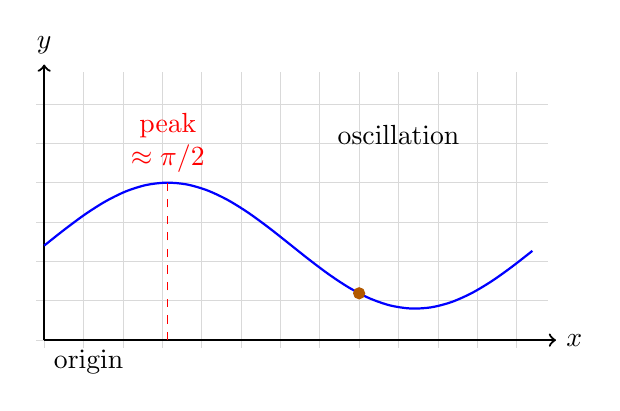
\begin{tikzpicture}[scale=1.0]
    \draw[step=0.5cm,gray!30,very thin] (-0.1,-0.1) grid (6.4,3.4);
    \draw[->,thick] (0,0) -- (6.5,0) node[anchor=west] {$x$};
    \draw[->,thick] (0,0) -- (0,3.5) node[anchor=south] {$y$};
    \draw[domain=0:6.2,smooth,variable=\x,blue,thick] plot ({\x},{1.2 + 0.8*sin(\x r)});
    \draw[dashed,red] (1.57,0) -- (1.57,2) node[above,align=center]{peak\\$\approx \pi/2$};
    \node[below right] at (0,0) {origin};
    \node at (4.5,2.6) {oscillation};
    \filldraw[orange!70!black] (4,{1.2 + 0.8*sin(4 r)}) circle (2pt);
  \end{tikzpicture}
  \caption{Sine-like curve with annotations and grid.}
\end{figure}

\newpage
\section{Paragraph Stress Test}
Continuous prose with mixed punctuation: ``Edge-aware OCR systems must balance recall and precision; however, noise---especially from compressed scans---can create artifacts.'' The quick brown fox jumps over the lazy dog. A second paragraph repeats with minor edits to detect hallucination: the quick brown fox jumps over the lazy dog, but this time the fox pauses at line breaks to test robustness.

\section{Code Fragment}
Verbatim text can challenge OCR because of monospaced glyphs:
\begin{verbatim}
for (int i = 0; i < 5; ++i) {
    double w = exp(-0.5 * pow(i - 2.0, 2));
    printf("w[%d] = %.3f\n", i, w);
}
\end{verbatim}

\section{Conclusion}
This concludes the synthetic PDF. Inspect the extracted text for dropped symbols, merged lines, and mis-ordered sections. Compare the OCR output with the known ground truth here to quantify accuracy.

\end{document}
